\chapter{Παράρτημα}
\label{chapter:appendix}

\begin{appendices}
    \section*{Παράρτημα Α: Επεκτάσεις Θεωρίας}
    \subsubsection{Πολυώνυμα Bernstein}
    Για κάθε φυσικό αριθμό $n \in \mathbb{N}$ , η πολυωνιμική συνάρτηση $\phi(\tau)$ ή χρησιμοποιώντας το σύμβολο $B(\tau)$ για τα πολυώνυμα Berstein, δίνεται από την μορφή:
    \begin{equation}
        B_k^n(\tau):=\left(\begin{array}{l} n \\k \end{array}\right) \tau^k(1-\tau)^{n-k},   \forall k \in [0,n]
        \label{eq:BersteinPolynomials}
    \end{equation}

    \subsubsection{Προσέγγιση Bézier - Bernstein}
    Τα πολυώνυμα Bernstein $B_k^n(\tau)(\tau;\Vec{\alpha})$, όπου το διάνυσμα $\Vec{\alpha} = (\alpha_1,\alpha_2,...\alpha_n)$ είναι μια ακολουθία παραμέτρων, εισάγουν την έννοια των βαθμών ελευθερίας μπορούν να προσεγγίσουν με την μέθοδο Bézier καμπύλες και επιφάνειες ως ανάπτυγμα αυτών των παραμετροποιημένων όρων  με την παρακάτω μορφή με βάση τις \ref{eq:PolynomialBaseSeries}, \ref{eq:BersteinPolynomials} : 
    \begin{equation*}
        \mathbf{P}(t)=\sum_{i=0}^n \mathbf{p}_i B^{i}_{n}(t), \quad 0 \leq t \leq 1
    \end{equation*}

    \begin{figure}[!tbh]
    \centering
    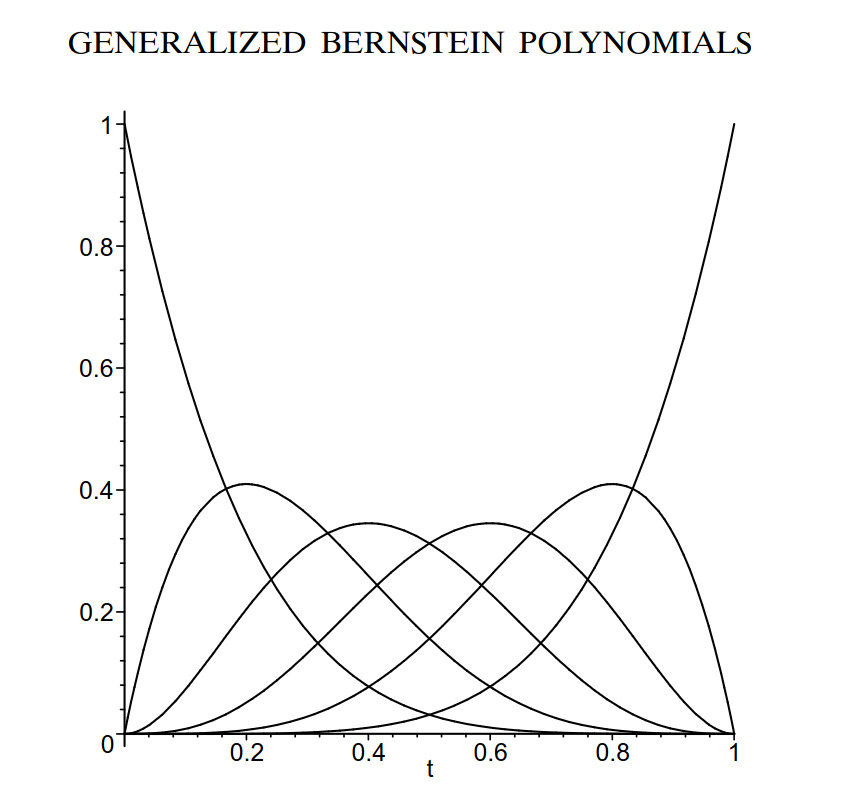
\includegraphics[width=5.5cm]{images/chapter2_img/GenerelizedBersteinPolynomials.jpg}
    \caption{Γενικευμένα Πολυώνυμα Bernstein $5^{ου}$ βαθμού ${B_{k}}^{5} $ στο [0,1]. Πηγή \cite{winkel2001generalized}}
    \label{fig:2 Generalized Bernstein Polynomials}
    \end{figure} 
    Συνήθως αυτή με αυτή την μεθοδολογία προσεγγίζονται καμπύλες τμηματικά, δηλαδή σε περιοχές που ελέγχονται από 4 σημεία ελέγχου( n=3).
    \subsubsection{Πολυώνυμα Spline}
    Μια άλλη οικογένεια πολυωνιμικών συναρτήσεων βάσης είναι τα πολυώνυμα Bsplines των οποίων ο τύπος για m βαθμού είναι ο εξής:
    \[
        \phi_{k, 0}^{B S}(t)= \begin{cases}1 & t_k \leq t<t_{k+1} \\ 0 & \text { αλλού }\end{cases}
    \]
    και απαιτείται η επιλογή n + m + 2 διακριτών τιμών της τιμής $t$ έτσι:
    \[
        \phi_{k, m}^{B S}(t)=\frac{t-t_k}{t_{k+m}-t_k} \phi_{k, m-1}^{B S}(t)+\frac{t_{k+m+1}-t}{t_{k+m+1}-t_{k+1}} \phi_{k+1, m-1}^{B S}(t), \quad k=0, \ldots, r
    \]
    επομένως ισχύει η ακόλουθη έκφραση:
    \[
        \phi_{k, m}^{B S}\left(t_k\right)=\phi_{k, m}^{B S}\left(t_{k+m+1}\right)=0, \quad n \geq 1 .
    \]
    για αυτό οι τιμές $t_k$ είναι αποκαλούνται και δεσμοί των καμπυλών.
    Με την προσέγγιση Bezier παίρνουμε ανάλογα αναπτύγματα των αναπτυγμάτων Bezier Bernstein που είναι σε θέση να γενικεύσουν την ικανότητα αναπαράστασης οδηγώντας σε γενικευμένες καμπύλες Bspline.
    \subsection*{Μοντέλα Προβολής | Κάμερα και Θέαση}
    \label{appendix:camerasystem}
    \par
       Ένα σχετικά αφαιρετικό αλλά περιεκτικό διάγραμμα που παρουσιάζει την πλήρη γραμμή παραγωγής γραφικών φαίνεται παρακάτω \ref{fig:graphicsenginepipeline}:
        \begin{figure}[H]
        \centering
        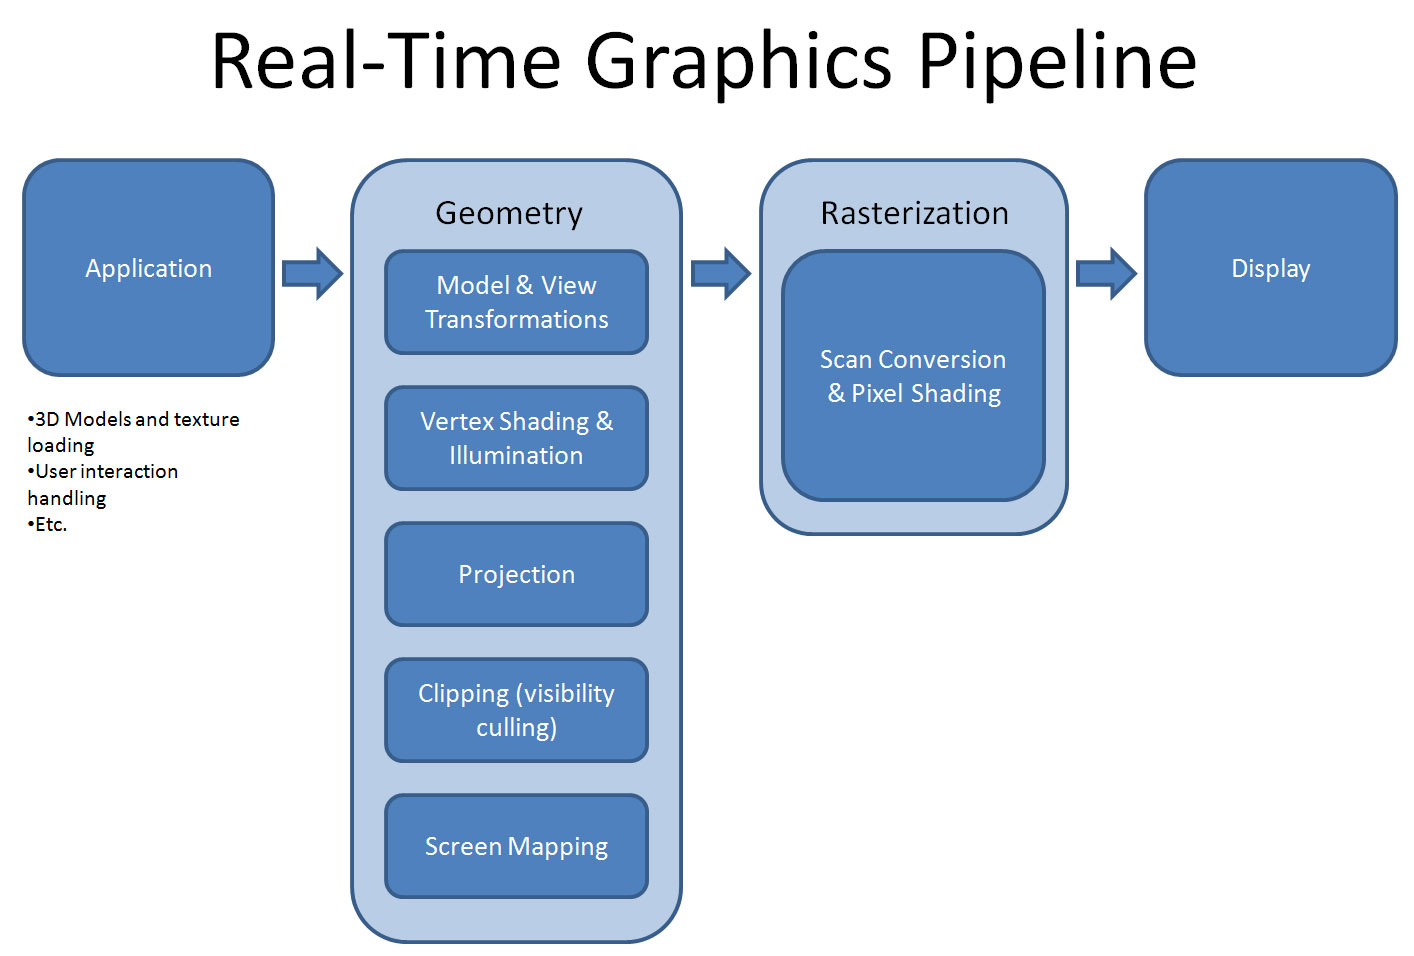
\includegraphics[width =.7\linewidth]{images/chapter2_img/pipeline.jpg}
        \caption{Βασική Γραμμή Παραγωγής Γραφικών }
        \label{fig:graphicsenginepipeline}
        \end{figure}
    Το κομμάτι των μετασχηματισμών αναφέρεται σε όλους του μετασχηματισμούς περιστροφής, και τους μετασχηματισμούς μετατόπισης αλλά και κλίμακας που εφαρμόζονται στα γραφικά πριν την προβολή τους.\\
    \par
        Συγκεκριμένα όσον αφορά την εργασία γίνεται εκτενής χρήση μεθόδων απόδοσης που βασίζονται στην ιχνηλάτιση ακτίνας καθώς και χρήση εικόνων για την εκτίμηση σφάλματος του δικτύου οπότε είναι επιτακτικό να γνωρίζουμε την βασική γραμμή παραγωγής σκηνών μέσω μηχανών γραφικών
        Στα πλαίσια της γραφικής υπολογιστών όταν γίνεται λόγος για απόδοση γραφικών αυτό αφορά και την προβολή τους σε κάποιο μέσο αναπαραγωγής. Τα ανθρώπινα μάτια δεν είναι σε θέση να δουν τρισδιάστατη πληροφορία κάτι που πηγάζει από τον τρόπο λειτουργίας τους. Συγκεκριμένα αυτό που αποτυπώνεται σε κάθε μάτι είναι ένα ανεστραμμένο είδωλο της \enit{3D} πληροφορίας ως μια εικόνα που ερεθίζει το οπτικό μας νεύρο. Η αντίληψη της τρισδιάστατης υπόστασης του χώρου είναι μια εμπειρική ικανότητα που οφείλεται στην απόσταση των ματιών μας (τεχνική που ακολουθείται και από κάμερες βάθους) αλλά κυρίως από άλλες αισθήσεις μας. 
    \begin{figure}[!tbh]
        \centering
        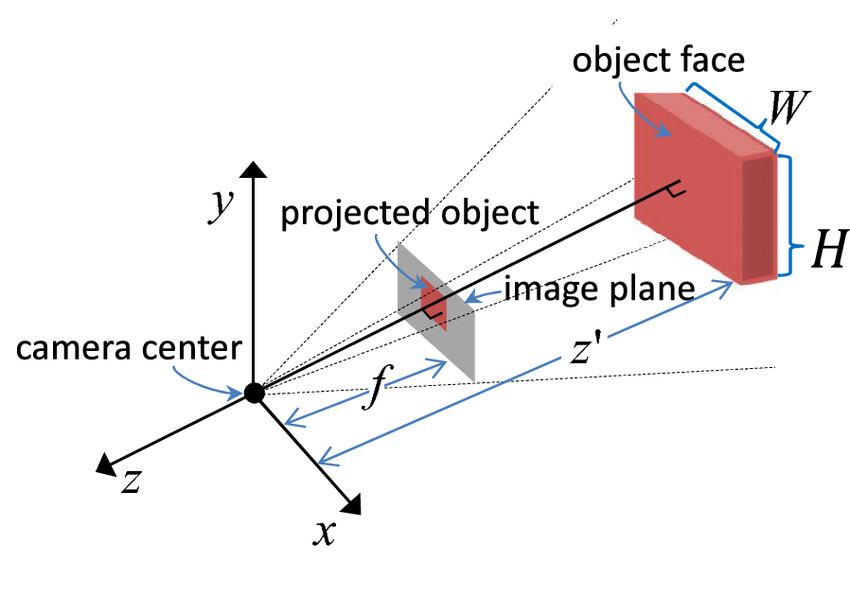
\includegraphics[width=.5\linewidth]{images/chapter2_img/Diagram-of-perspective-camera-model-in-3D.jpg}
        \caption{Σύστημα προοπτικής Προβολής \cite{article}}
        \label{fig:perspectiveProjection}
    \end{figure}
    Η διαδικασία παραγωγής μιας απεικόνισης γραφικών μιας τρισδιάστατης σκηνής είναι κάπως ανάλογη με τις διαδικασίες που σχετίζονται με την λήψη φωτογραφίας. Επί της ουσίας εισάγουμε ένα μοντέλο εικονικής κάμερας που παίζει τον ρόλο των ματιών του παρατηρητή και έχουμε δύο είδη προβολών. Την ορθογραφική η οποία δεν κάνει χρήση του πόσο κοντά είναι το αντικείμενο στην κάμερα και την προοπτική που δίνει την αίσθηση της μείωσης βάθους καθώς το αντικείμενο απομακρύνεται από την θέση της κάμερας. Το συνολικό μοντέλο προβολής πάνω στο πέτασμα της κάμερας όπου φαίνονται και σημαντικές παράμετροι της κάμερας (εσωτερικές, εξωτερικές ή όπως αναφέρεται στην διεθνή βιβλιογραφία \enit{intristic}, \enit{extrinsic}.
    \begin{figure}[!tbh]
        \centering
        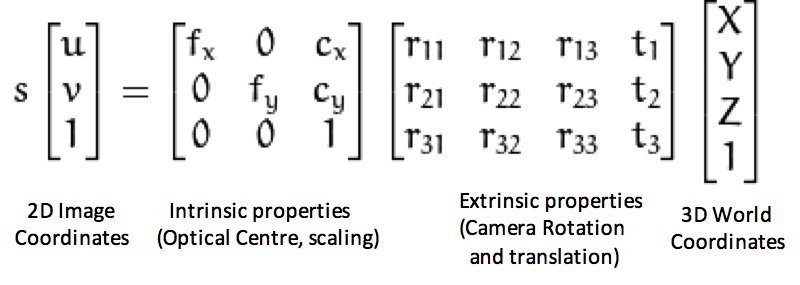
\includegraphics[width=0.4\linewidth]{images/chapter2_img/camera_properties_projection_system.jpg}
        \caption{εξωτερικές και εξωτερικές παράμετροι κάμερας σε μαθηματική μορφή συστήματος προβολής}
        \label{fig:intristicsextristics}
    \end{figure}
    
    Ο χώρος συντεταγμένων UV είναι ο χώρος των εικονοστοιχείων της εικόνας. Οι εξωτερικές παράμετροι αφορούν τον προσανατολισμό και την θέση της κάμερας ενώ οι εξωτερικές παράμετροι αφορούν το μήκος του φακού δηλαδή το ποσό της προοπτικής κλιμάκωσης καθώς και το οπτικό κέντρο. Όταν γίνεται λόγος για φωτογραφική ομοιότητα μιλάμε για το πόσο ίδιες είναι οι σκηνές υπό το πρίσμα της απόστασης σε τιμή φωτεινότητας (σε όλα τα κανάλια πχ. [R, G, B]) των εικονοστοιχείων στο UV επίπεδο.


    \subsection*{Τρόπος αναπαράστασης και αρχικοποίησης καμερών στην εργασία}
    \label{appendix:camerainitrepresent}

    Μια κάμερα αναπαριστάται με ένα σύνολο  διανυσμάτων \(\mathcal{C} = (\boldsymbol{q},c,\boldsymbol{K})\) όπου το \(\boldsymbol{q} \in \mathbb{R}^4\) είναι το \enit{quaternion} διάνυσμα \footnote{τα \enit{quternions} ή τετραδρόνια είναι αναπαραστάσεις διανυσμάτων τεσσάρων διαστάσεων που επεκτείνουν το σύστημα των μιγαδικών αριθμών και χρησιμοποιούνται συχνά σε εφαρμογές ρομποτικής και γραφικής σε ομογενείς μετασχηματισμούς (στροφές) όπου δεν ισχύουν αντιμεταθετικές ιδιότητες}, το οποίο αναπαριστά την πόζα ή στροφή της κάμερας, \(\boldsymbol{c} \in \mathbb{R}^3\) αναπαριστά την θέση της κάμερας, και \(\boldsymbol{K} \in \mathbb{R}^{3 \times 3}\) αναπαριστά τον πίνακα εσωτερικών παραμέτρων της κάμερας.

    Οι παράμετροι της κάμερας είναι οι \(\tau = \mathcal{(C}_{1}\mathcal{, .... , C_{N})}\), όπου \(N\) ο αριθμός των καμερών (και ταυτοχρόνως και εικόνων όψης του  αντικειμένου). Έστω \(\boldsymbol{Q(q)} \in \mathbb{R}^{3\times 3}\) συμβολίζει τον πίνακα στροφής που αντιστοιχεί στο \enit{quaternion} \(\boldsymbol{q}\). Τότε, για την κάμερα \(\mathcal{C}_{i}, i \in [N]\), και για pixel u έχουμε:

    \begin{equation}
        c_u(\tau) = c_i,
        \label{eq:camerapos}
    \end{equation}
    \begin{equation}
        \boldsymbol{w}_u(\tau) = \frac{1}{||\boldsymbol{K_{i}}^{-1}u||_{2}}\boldsymbol{Q(q_i)K_{i}^{-1}u},
        \label{eq:viewdir}
    \end{equation}
    όπου το \(\boldsymbol{u} = (u_{x},u_{y},1)^{T}\) είναι το pixel u σε ομογενής συντεταγμένες.


    Στα πειράματα που πραγματοποιήθηκαν, σε περιπτώσεις που οι παράμετροι κάμερας για μια σκηνή που αντιστοιχεί σε ένα \enit{3D} αντικείμενο δεν υπάρχουν, δημιουργούνται σχετικές μετακινήσεις μεταξύ ζευγαριών κάμερα χρησιμοποιώντας τον αλγόριθμο \enit{SIFT feature matching} \cite{lowe2004distinctive} και ένας ανθεκτικός στατιστικά πίνακας εκτίμησης (RANSAC), ο οποίος ακολουθείται από την αποσύνθεση των σχετικών περιστροφών και μετατοπίσεων μεταξύ των καμερών \cite{hartley2003multiple}. Οι σχετικές μετακινήσεις ως είσοδοι στην γραμμική μέθοδο κανονικοποίησης που χρησιμοποιείται \cite{jiang2013global} παράγει κάμερες με θόρυβο. Θεωρούνται γνωστοί οι παράμετροι της κάμερας όπως συχνά θεωρείται και το SFM \cite{schonberger2016structure}.
    
    \subsection*{Μοντέλο Phong Φωτισμού - P-Universal Renderer}
    \label{appendix:phong}
    Στην θεωρία γραφικής υπολογιστών ο φωτισμός είναι ένα μεγάλο κεφάλαιο. Η μεθοδολογία που ακολουθείται είναι η συνολική εκτίμηση όλων των μορφών του φωτισμού και ο υπολογισμός της επίδρασης που έχουν στο χρώμα. Οι μορφές φωτισμού που υπάρχουν επηρεάζονται ιδιαιτέρως από την υφή της επιφάνειας δηλαδή την κατανομή των κανονικών διανυσμάτων στα πιο σύνθετα μοντέλα φωτισμού όπως ο η κατοπτρική ανάκλαση και ο περιορισμός του πεδίου φωτός που επιβάλουν οι συντελεστές Phong.
    \begin{figure}[H]
        \centering
        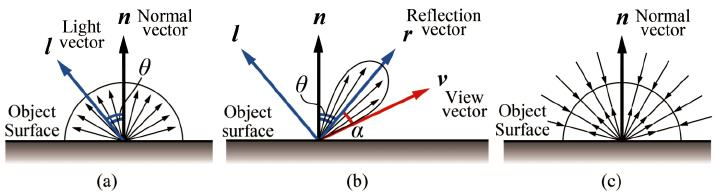
\includegraphics[width = 0.6\linewidth]{images/chapter2_img/Phong-reflection-model-a-diffuse-b-specular-light.jpg}
        \caption{ Διανύσματα,Διάχυτη Ανάκλαση, Κατοπτρικό Ανάκλαση, Μοντέλο Ανάκλασης Phong, Πηγή \cite{shader-hologram}}
        \label{fig:PhongReflectionmodel}
    \end{figure}
    Όπως φαίνεται και στο σχήμα \ref{fig:PhongReflectionmodel}, ανάλογα το είδος του φωτισμού που μελετάμε μας ενδιαφέρουν διαφορετικά διανύσματα είτε πρόσπτωσης(φως διάχυσης) είτε ανάκλασης(κατοπτρικής ανάκλαση) στην επιφάνεια. Σε όλα τα μοντέλα όμως είναι απαραίτητη η επίγνωση του κανονικού διανύσματος στην επιφάνεια. Το μοντέλο Phong συνδυάζει όλα τα μοντέλα φωτισμού  περιλαμβάνοντας και παραμέτρους  για την υφή των υλικών η οποία. Συνολικά η περιγραφή του  περιορισμένου μοντέλου φωτισμού για δοθέν σημείο πρόσπτωσης \(\hat{x}\) και διάνυσμα ανάκλασης \(\boldsymbol{w}^o\) δίνεται από την εξίσωση:
    \begin{equation}        
        L(\hat{x},\boldsymbol{w}^o) = k_{d}O_{d}I_{\alpha} + k_{d}O_{d}I_{d}(\hat{n} \cdot \frac{\boldsymbol{l}- \hat{x}}{||\boldsymbol{l} - \hat{x}||}) + k_{s}O_{s}I_{d}(\hat{r}\cdot \frac{\boldsymbol{l}- \hat{x}}{||\boldsymbol{l} - \hat{x}||})^{n_{\text{phong}}},
        \label{eq:PhongReflectionModel}
    \end{equation}

    με $\alpha$ να είναι το μήκος κύματος διάχυτης ακτινοβολίας, $k_d, k_s$ συντελεστές διάχυτης και κατοπτρικής ανάκλασης, $I_a,I_d$, το διάχυτο φως το φως σημειακής πηγής(χρώμα πηγής) και $O_d,O_s$, είναι τα χρώματα της επιφάνειας. Η θέση της σημειακής πηγής καθορίζεται από το $\boldsymbol{l} \in \mathbb{R}^3$ και $\boldsymbol{w^o} = -\boldsymbol{w}$ δηλαδή το διάνυσμα ανάποδο από το διάνυσμα όψης ή $\boldsymbol{v}$ όπως φαίνεται στο σχήμα \ref{fig:PhongReflectionmodel}. Το διάνυσμα ανάκλασης \(\hat{r}\) δίνεται από τον νόμο ανάκλασης \(\hat{r} = -(I - 2\hat{n}\hat{n}^T)\boldsymbol{w}^o\) σε συνάρτηση του κανονικού διανύσματος. Ο συντελεστής $n_{phong}$ είναι ο συντελεστής του κατοπτρικού μοντέλου Phong που αλλάζει τα κατοπτρικά φαινόμενα στο χρώμα.

    Η οικογένεια αυτή δεν περιλαμβάνει όλα τα στοιχεία φωτισμού, παραδείγματος χάρη δεν υπολογίζει σκιές από το ίδιο το σώμα που φωτίζεται, αφού για δεύτερη ή υψηλότερη παράγωγο του L η γεωμετρία δεν παίζει ρόλο στον υπολογισμό του χρώματος.

    Η έρευνα χρησιμοποιεί μια συνάρτηση για να περιγράψει όλα αυτά τα μοντέλα φωτισμού την \(\mathcal{M}(x,n,\boldsymbol{w};\gamma)\) όπου M είναι ένα MLP δίκτυο. Η συνεχή αυτή συνάρτηση που προσεγγίζει το δίκτυο μπορεί να περιγράψει πληροφορία για πλήθος φωτισμών μεγιστοποιώντας το διάνυσμα εξόδου σε συνάρτηση με τις παραμέτρους γ της εμφάνισης. Αυτό βασίζεται στην παρακάτω θεωρία του πως ένα MLP δίκτυο που περιγράφει Level Set πολλαπλότητες μπορεί να αναπαραστήσει οποιαδήποτε τμηματικά συνεχή συνάρτηση μεγιστοποιώντας ένα διάνυσμα εισόδου. Στην συγκεκριμένη περίπτωση το διάνυσμα εισόδου περιλαμβάνει τα κάθετα διανύσματα οπότε αποτυπώνονται κατοπτρικά φαινόμενα. Πρακτικά περιγράφεται η επιφανειακή κατανομή χρώματος ή Texture. Τότε το δίκτυο ονομάζεται P-Universal Renderer.

    \section*{Παράρτημα Β: Αποδείξεις}
    \begin{theorem}{Θεώρημα αναπαράστασης συμπαγών επιφανειών μέσω ελεγχόμενων νευρωνικών επιπέδων}
        Κάθε συμπαγής, όχι αναγκαστικά φραγμένη, τμηματικά γραμμική υπερεπιφάνεια ${M} \subset \mathbb{R}^d$  μπορεί να αναπαρασταθεί με ακρίβεια, ως ένα νευρωνικά διαφορίσιμη πολλαπλότητα (τοπολογία,ισομετρική επιφάνεια) ${S}$ ενός πολυστρωματικού perceptron δικτύου με ReLU συναρτήσεις ενεργοποίησης,
        ${F}:\mathbb{R}^d \rightarrow \mathbb{R}$. 
    \end{theorem}
    \begin{proof}
        Έστω $h_i(x) = a_{i}^T x + b_{i} =  0\, i \in [k]$  συμβολίζει την επιφάνεια η οποία υποστηρίζεται από τις έδρες του ${M}$ όπου τα $a_i$ είναι επιλεγμένα ώστε να είναι τα προς τα έξω κανονικά διανύσματα της επιφάνειας σε αυτές τις έδρες. Εφόσον η ${M}$ είναι συμπαγής δηλαδή αποτελεί \enit{Convex Hull} ή κυρτή τοπολογία του χώρου, αποτελεί ένα φράγμα d-διάστατου χώρου ${P}$.

        Για κάθε \(\lambda \in {-1,0,1}^{k}\), έστω \({P_\lambda} = \cap_{i \in [k]}\{x | \lambda_{i}h_{i}(x) \geq 0 \}\). Πιο απλά, \({P_\lambda}\) είναι ένας χώρος όπου κάθε τομή κλειστών ημι-χώρων ορίζεται από κάποιο από τα υπερεπίπεδα \(h_i\). Από όλα τα \({P}_\lambda\), μας ενδιαφέρει αυτά που περιέχονται στο \({P}\), έτσι ορίζεται \(\Lambda = \{\lambda | {P_\lambda} \subseteq {P}\}\). Έτσι τώρα, αρκεί να δείξουμε ότι κάθε σημείο στο εσωτερικό μια μεγάλης τοπολογίας βρίσκεται και αυτό αναγκαστικά εσωτερικά κάποιων μικρών τοπολογιών στην συλλογή, δηλαδή \(\cup_{\lambda \in \Lambda} \mathring{{P_{\lambda}}} = \mathring{{P}}\). Έτσι για δεδομένο $x \in \mathring{P}$ υπάρχουν δύο περιπτώσεις στο που μπορεί να βρίσκεται:

        Περίπτωση 1: \(h_{i} \neq 0 \forall i \in [k]\). Δεδομένου αυτού το, $x$ δεν βρίσκεται ακριβώς σε κάποιο υπερεπίπεδο. Μπορούμε να πάρουμε τις υπόλοιπες πολυδιάστατες τοπολογίες \(P_{\lambda}\) οι οποίες περιέχουν εσωτερικά το \(x\) θέτοντας: \(\lambda_{i} = sign(h_{i}(x))\). Σημειώνεται ότι, \(\lambda \in \{-1,1\}^{k}\), και για αυτές τις τιμές η πολυδιάστατη τοπολογία που αναπαρίσταται λέγεται ελάχιστη (\enit{minimal}). Διατυπώνεται ο ισχυρισμός ότι η ελάχιστη τοπολογία είναι στο εσωτερικό ή εντελώς εξωτερικά στο σύνολο \(P\). Αυτό επιβεβαιώνεται καθώς σε άλλη περίπτωση, η ελάχιστη τοπολογία θα περιείχε δύο σημεία τα οποία βρίσκονται σε διαφορετικές πλευρές κάποιου υπερεπιπέδου, το οποίο δεν συμβαδίζει για τις τιμές του $\lambda \in \{-1, 1\}^k$. Συνεπώς στην περίπτωση μας, ξέρουμε ότι $P_{\lambda}$  και $P$ περιέχουν το $x$ ως εσωτερικό σημείο, και αυτό σημαίνει ότι απαραίτητα $P_{\lambda} \subseteq P$ άρα και $\lambda \in \Lambda$.

        Περίπτωση 2: \( \exists \{i_1,...,i_l\} \subseteq [k]\) τέτοιο ώστε \(h_{i}(x) = 0 \forall i \in  \{i_1,...,i_l\}\), και $h_i \neq 0 \forall i \in [k] \ \{i_1,...,i_l\}$. Σε αυτή την περίπτωση, δεν υπάρχει ελάχιστη τοπολογία η οποία να περιέχει το $x$ εσωτερικά της. Έτσι ας υποθέσουμε ότι τις όλες οι ελάχιστες τοπολογίες οι οποίες περιέχουν το $x$  στο όριο τους. Έστω \(P_{u}\) μια τέτοια ελάχιστη τοπολογία πολλών διαστάσεων. Όπως προαναφέρθηκε, το εσωτερικό \(P_{u}\) της είναι είτε εντελώς εντός του συνόλου τροπολογιών \(P\) ή εντελώς εκτός, αλλά αφού το \(x\) είναι ταυτόχρονα στα όρια της \(P_{u}\) και εντός της \(P\), αναγκαστικά η \(P_{u}\) είναι εσωτερικά της \(P\), δηλαδή \(P_{u} \subset P\). Μας ενδιαφέρει το σύνολο όλων αυτών των ελάχιστων τοπολογιών. Σημειώνεται πως για τέτοια ελάχιστη τοπολογία, \(P_{u}\), αναγκαστικά $u_{i} = sign(h_i(x)) \forall i  \in [k] \ \{i_1,...,i_l\} $. Για \(i \in \{i_1,...,i_l\}\), το \(u_i\) μπορεί να πάρει τιμές στο \( \{1, -1\} \). Έτσι, η ένωση όλων αυτών των ελάχιστων τοπολογιών είναι οι \(P_{\lambda}\) όπου:\[\lambda_i =
                        \begin{cases}
                        0, & \text{if } i \in \{i_1, \ldots, i_l\} \\
                        \text{sign}(h_i(x)), & \text{αλλού}
                        \end{cases}
                    \]
        οι οποίες προφανώς περιέχει το σημείο $x$ στο εσωτερικό τους και οι ίδιες περιέχονται στο \(P\) (ως ένωση τοπολογιών που περιέχονται στο \(P\)), δηλαδή \(\lambda \in \Lambda\).

        Έχοντας δείξει τα παραπάνω μπορούμε να ορίσουμε μια συνάρτηση η οποία δέχεται θετικές τιμές στο εσωτερικό του συνόλου \(P\), αρνητικές τιμές στο εξωτερικό του \(P\) (ή μπορεί και ανάποδα ανάλογα την σύμβαση). Έτσι ορίζεται συνάρτηση πολλαπλότητας:
        \[
            f(x) = \max_{\lambda \in \Lambda} \min_{i \in [k]} \lambda_{i}h_{i}(x)
        \]
        Η f, είναι τμηματικά συνεχής συνάρτηση, συνεπώς, με βάση το θεώρημα μπορεί να κωδικοποιηθεί ως δίκτυο MLP με συναρτήσεις ενεργοποίησης ReLU. Η συνολική ιδέα βασίζεται στην δημιουργία τελεστών max χρησιμοποιώντας γραμμικά στρώματά και ReLU δηλαδή $\text{max} \{a, b\} = \sigma(a - b)^2 + \sigma(b - a)^2 + (a + b)^2$, όπου $\sigma(x) = \max(0, x) $ η συνάρτηση ReLU. Χρησιμοποιώντας αυτούς τους δυαδικούς τελεστές μπορεί κανείς να δημιουργήσει τον μέγιστο ενός διανύσματος και το ελάχιστο με τον ιδιο τροπο προσεγγίζοντας οποιαδήποτε τοπολογία.

    \end{proof}\cite{DBLP:journals/corr/abs-1905-11911}
   
    
    \section*{Παράδειγμα Γ: Ενδεικτικοί Αλγόριθμοι που Υλοποιήθηκαν ή Aναφέρονται }

        
        \label{section:appendix-algorithms}

        \subsection*{Αλγόριθμος Νευρωνικής Κωδικοποίησης Κατακερματισμού Hash - Multi-Resolution HashGrid3D Encoding}
        \begin{algorithm}[H]
            \caption{HashGrid3D-Neural Coordinate Encoding}
            \begin{algorithmic}
                \State Ορισμός σταθερών: $\pi_{i}$.
                \State Ορισμός ενός πίνακα πρώτων αριθμών HASH\_PRIMES.
                
                \Procedure{HashGrid3D}{\textbf{d}, \textbf{F}, \textbf{$\log(T)$}, \textbf{$N_{\ell}$}}
                
                    \State \small{Αρχικοποίηση του HashGrid3D με τις διαστάσεις εισόδου, μέγεθος τιμών κατακερματισμού, μέγεθος χάρτη και ανάλυση}.
                    \State \small{Δημιουργία πίνακα αναζήτησης για τιμές κατακερματισμού $T$}.
                    \State \small{Αρχικοποίηση μάσκας διασταύρωσης \enit{Binary Mask}}.
                    \State \small{Αρχικοποίηση βαρών EmbeddingLayer με ομοιόμορφη κατανομή μικρής τυπικής απόκλισης}.
                
                \EndProcedure
                
                \Procedure{HashGrid3Dforward}{x, υπολογισμός\_κλίσης}
                    \State $x_i = \lfloor x \rfloor$.
                    \State $x_f = x_i - x.float()$   \Comment{\small{Κλιμάκωση εισόδου στην δοθείσα ανάλυση}}.
                    \State \textbf{neighbors = bin\_mask($x_i, x_i + 1$)}
                    \State\textbf{w\_ids = bin\_mask$(1 - x_f, x_f)$} \Comment{
                \small{Υπολογισμός γειτόνων, παρεμβολή των δεδομένων των γειτόνων στην δοθείσα ανάλυση}}.
                    \State Εφαρμογή συνάρτησης hash στα ids των γειτόνων και αντιστοίχηση τους σε βάρη του δικτύου προσοχής.
                    \State \textbf{neig\_hash\_data = EmbeddingLayer(hash\_func(w\_ids, HASH\_PRIMES, $T$)) }
                    \State Επέστρεψε $\sum{neig_{data}*w_{ids}*w_{ids}^{T}}$ \Comment{\small{Παρεμβολή των δεδομένων των γειτόνων}}.
                \EndProcedure
                
                \Procedure{\textbf{MultiResHashGrid3D}}{\textbf{includeInput}, \textbf{d}, \textbf{L}, \textbf{F}, \textbf{$\log(T)$}, \textbf{$N_{min}$}, \textbf{$N_{max}$}}
                \State Αρχικοποίηση MultiResHashGrid3D με παραμέτρους.
                \State Υπολογισμός  $N_{\ell}:=\left\lfloor N_{\min }\cdot b^{\ell}\right\rfloor$
                \State Δημιουργία Πολλαπλής Ανάλυσης Πλεγμάτων με κλήση  HashGrid3D.
                \If{\textbf{includeInput}}
                   \State Αρχικοποίηση FourierFeatureNTK για κωδικοποίηση Βοηθητικής εισόδου.
                \EndIf
                \EndProcedure
                
                \Procedure{MultiResHashGrid3Dforward}{x, υπολογισμός\_κλίσης}
               
                \State Συγχώνευση των πλεγμάτων κωδικοποίησης από κάθε επίπεδο ανάλυσης.
                \If{\textbf{includeInput}}
                 \State Συγχώνευση FFNTK(x), MultiResHashGrid3D(x).
                \EndIf
                \State Επιστροφή συγχωνευμένου διανύσματος χαρακτηριστικών
                \EndProcedure
            \end{algorithmic}
        \end{algorithm}
        Στο \enit{backward pass} του δικτύου επιστρέφονται σφάλματα μέχρι τα βάρη των γειτόνων και ρυθμίζονται οι παράμετροι του \enit{Embedding} στρώματος νευρώνων. Αυτά αντιστοιχούν με  \enit{Lookup Table} στα διακριτά χαρακτηριστικά των γειτονικών \enit{hash}, μετατρέποντας την διαδικασία από διακριτό μετασχηματισμό σε γραμμικό. Με αυτό τον τρόπο επιτρέπεται η εκπαίδευση των κωδικοποιήσεων των συντεταγμένων/διανυσμάτων όψης σε συνάρτηση με την αξιοπιστία \enit{3D} ανακατασκευής.
        \subsection*{Χρήση Δικτύου LSTM για τον υπολογισμό των μήκους των πεπερασμένων βημάτων}
            (Από το κεφάλαιο \textit{Μέθοδοι Απόδοσης - Ray Marching} \ref{section:rendering})
            Πολλές φορές είναι θεμιτό να βελτιστοποιηθούν όσο τον δυνατόν περισσότερο χρονοβόροι αλγόριθμοι που εκτελούν απόδοση γραφικών. Στην περίπτωση του \enit{Ray Marching} αυτό γίνεται εφικτό με έναν περιορισμό στο πλήθος τον βημάτων που γίνονται προς μια κατεύθυνση. Ωστόσο, δεν είναι γνωστές οι διαστάσεις της σκηνής, ο χώρος ο οποίο αναπαρίσταται δηλαδή, η επιλογή του βήματος βάδισης δηλαδή του μήκους το οποίο θα διανύσει μια ακτίνα για να ελέγξει ξανά την απόστασή της από την έμμεση επιφάνεια, μπορεί να μην είναι ιδανική. Η επιστημονική κοινότητα εξελίσσοντας τα δίκτυα LSTM δηλαδή Long Short Term Memory το οποίο αναπαριστώντας διάφορες σκηνές από διάφορες όψεις ενός χώρου είναι σε θέση να εκτιμήσει το ιδανικό μήκος βήματος $\delta$ και να το εισάγει στον αλγόριθμο δίνοντας καλύτερα αποτελέσματα σε λιγότερο χρόνο. Στο κομμάτι της εργασίας δεν υιοθετείται LSTM εκδοχή του δικτύου \enit{ray tracing}, ωστόσο είναι μια καλή βελτιστοποίηση που θα μείωνε τον χρόνο απόδοσης της σκηνής σε εικόνα.
            \begin{algorithm}[ht]
            \caption{Ray Marching Algorithm using LSTM step length Prediction}
            \begin{algorithmic}
            \Function{RayMarch}{$\Phi, K, E, (u, v)$}
            \State $d_0 \gets 0.05$ \Comment{Near plane}
            \State $(h_0, c_0) \gets (0, 0)$ \Comment{Initial state of LSTM}
            \For{$i \gets 0$ \textbf{to} $max\_iter$}
                \State $x_i \gets r_{u,v}(d_i)$ \Comment{Calculate world coordinates}
                \State $v_i \gets \Phi(x_i)$ \Comment{Extract feature vector}
                \State $(\delta, h_{i+1}, c_{i+1}) \gets LSTM(v_i, h_i, c_i)$ \Comment{Predict steplength using ray marching LSTM}
                \State $d_{i+1} \gets d_i + \delta$ \Comment{Update $d$}
            \EndFor
            \State \textbf{return} $r_{u,v}(d_{max\_iter})$
            \EndFunction
            \end{algorithmic}
            \end{algorithm}
            \newline
            \clearpage
        \subsection*{Αλγόριθμος εξαγωγής Πλέγματος Τριγώνων από Έμμεση αναπαράσταση επιφάνειας | Marching Cubes}
        \par 
            Πλήθος μεθόδων από την δεκαετία του 80 ακόμα προσπάθησαν να μετατρέψουν τις έμμεσες αναπαραστάσεις γραφικών σε πλέγματα πολυγώνων με κάποια ανοχή στα σφάλματα και χωρίς βλάβη της γενικότητας, επιτρέποντας την χρήση των υπαρχόντων πολυγώνων. Το πρόβλημα αυτό ήρθε να λύση οριστικά δίνοντας την χρυσή τομή στο ισοζύγιο υπολογιστικής πολυπλοκότητας και ανάλυσης ο αλγόριθμος \enit{Marching Cubes}.
        \par
            \begin{figure}[H]
                \centering
                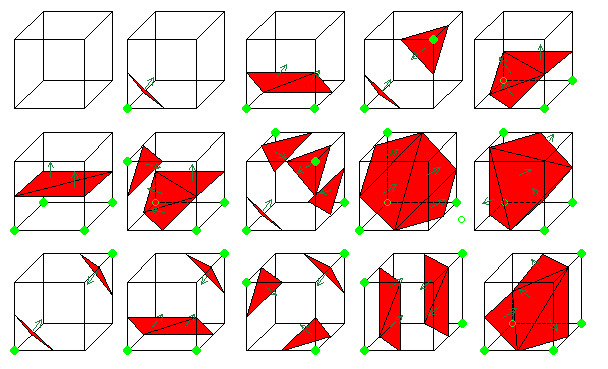
\includegraphics[width = 0.8\linewidth]{images/chapter2_img/marching_cubes.jpg}
                \caption{Απεικόνιση Lookup Table ανάλυσης 8,αλγορίθμου Marching Cubes}
                \label{fig:marchingcubes}
            \end{figure}
            Ο αλγόριθμος Marching Cubes\cite{marchingcubes}, στην τρισδιάστατη μορφή του κάνει χρήση της δομής του ογκομετρικού διαμερισμού του χώρου σε voxels. Τα βήματα που ακολουθεί είναι τα εξής:
           \begin{algorithm}[H]
            \caption{3D Marching Cubes Algorithm}
            \begin{algorithmic}
            \State \textbf{Classify grid nodes as inside/outside:}
            \For{each grid node $(x_{i,j,k})$}
            \State Is $F(x_{i,j,k}) > 0$ or $F(x_{i,j,k}) < 0$?
            \EndFor
            
            \State \textbf{Classify cell: $2^{resolution}$ configurations:}
            \For{each cell}
            \State In/out for each corner
            \EndFor
            
            \State \textbf{Compute intersection points:}
            \For{each edge}
            \State Linear interpolation along edges
            \EndFor
            
            
            \State \textbf{Connect them by edges:}
            \State Look-up table for path configuration
            \State Disambiguation by modified table [Montani '94]
            \end{algorithmic}
            \end{algorithm} 
            


\subsection*{Παράμετροι δικτύων}
    \subsubsection{Χρήση Δικτύου IDR}
    Το δίκτυο IDR\cite{yariv2020multiview} έχει παραμετροποιηθεί ώστε να χρησιμοποιεί το κάθε μοντέλο κωδικοποίησης με παραμέτρους που ορίζονται σε ένα αρχείο HOCON (JSON). Παράλληλα εκεί ορίζονται όλοι οι υπερπαράμετροι του δικτύου καθώς και αντίστοιχο αρχείο χρησιμοποιείται για την ρύθμιση του δικτύου σε άγνωστη θέση καμερών η οποία εκτιμάται και εκπαιδεύεται. Στα πλαίσια της εργασίας δεν κρίθηκε απαραίτητο να εκπαιδευτούν οι θέσεις των καμερών.

    Οι παράμετροι του IDR με τις οποίες εκπαιδεύτηκε είναι οι εξής:
       
        \begin{itemize}
            \item πλήθος pixel ανά batch, training\_pixel\_batch\_size = 2048
            \item ορόσημα παραμέτρου σύγκλισης μάσκας, $\alpha$-milestones = [250, 500, 750, 1000, 1250]
            \item αρχικό βήμα εκπαίδευσης, learning\_rate = 0.0001
            \item ποσοστό μείωσης του learning\_rate, sched\_factor = 0.5
            \item εποχές μείωσης του βήματος εκπαίδευσης, sched\_milestones = [1000, 1500]
            \item βάρος απόκλισης από την εικονική εξίσωση, eikonal\_weight = 0.1
            \item βάρος σφάλματος μάσκας, mask\_weight = 100 ή 200 στο NFFB
        \end{itemize}

        Παράμετροι δικτύων, Implicit Network
        \begin{itemize}
            \item διάσταση εισόδου, din = 3
            \item διάσταση εξόδου, dout = 1
            \item διαστάσεις κρυφών επιπέδων, dims = [512, 512, 512, 512, 512, 512, 512, 512]
            \item γεωμετρική κανονικοποίηση, geometric\_init = True
            \item bias βαρών, bias = 0.6
            \item διακοπή δικτύου στο επίπεδο 4, skip\_in = [4]
            \item κανονικοποίηση βαρών, weight\_norm = True
            \item Πλήθος Συχνοτήτων Κωδικοποίησης/Επιπέδων Βαθιάς Κωδικοποίησης = 6
        \end{itemize}
        Rendering Network \\
        \begin{itemize}
            \item διάσταση εισόδου, din = 9
            \item διάσταση εξόδου, dout=3
            \item Είδος κωδικοποίησης διανυσμάτων όψης, [Δικτυο κωδικοποίησης]
            \item  διαστάσεις κρυφών επιπέδων, dims = [ 512, 512, 512, 512]
            \item  κανονικοποίηση βαρών, 
            \item Πλήθος Συχνοτήτων Κωδικοποίησης/Επιπέδων Βαθιάς Κωδικοποίησης = 4
        \end{itemize} 
        Δίκτυο Βαθιάς Κωδικοποίησης NFFB\\ 
        \begin{itemize}
            \item Μέγεθος πίνακα Hash, $T = 10^{19}$
            \item Πλήθος χαρακτηριστικών ανά κελί $F =2$
            \item Αρχική Ανάλυση (low res) $N_0 = 16$
            \item Τελική Ανάλυση (coarse res) $N_{max} = 512$
            \item Συντελεστής κανονικοποίησης εισόδου, bound = 0.42
        \end{itemize}
        Κωδικοποίηση HashGrid3D\\ 
        \begin{itemize}
            \item Μέγεθος πίνακα Hash, $T = 10^{5}$
            \item Πλήθος χαρακτηριστικών ανά κελί $F =2$
            \item Αρχική Ανάλυση (low res) $N_0 = 8$
            \item Τελική Ανάλυση (coarse res) $N_{max} = 512$
            \item Συντελεστής κανονικοποίησης εισόδου, bound = 1.0
        \end{itemize}
       Κωδικοποίηση HashGrid3D\_TCNN\\ 
        \begin{itemize}
            \item Μέγεθος πίνακα Hash, $T = 10^{15}$
            \item Πλήθος χαρακτηριστικών ανά κελί $F =2$
            \item Αρχική Ανάλυση (low res) $N_0= 16$
            \item Τελική Ανάλυση (coarse res) $N_{max} = 512$
            \item Συντελεστής κανονικοποίησης εισόδου, bound = 1.0
        \end{itemize}
        Δίκτυο Βαθιάς Κωδικοποίησης StylemodNFFB\\ 
        \begin{itemize}
            \item Μέγεθος πίνακα Hash, $T = 10^{5}$
            \item Πλήθος χαρακτηριστικών ανά κελί $F =2$
            \item Αρχική Ανάλυση (low res) $N_0 = 16$
            \item Τελική Ανάλυση (coarse res) $N_{max} = 512$
            \item Συντελεστής κανονικοποίησης εισόδου, bound = 0.45
        \end{itemize}
         Δίκτυο Βαθιάς Κωδικοποίησης StylemodNFFB\_TCNN\\ 
        \begin{itemize}
            \item Μέγεθος πίνακα Hash, $T = 10^{19}$
            \item Πλήθος χαρακτηριστικών ανά κελί $F =2$
            \item Αρχική Ανάλυση (low res) $ N_0 = 16$
            \item Τελική Ανάλυση (coarse res) $N_{max} = 512$
            \item Συντελεστής κανονικοποίησης εισόδου, bound = 0.45
        \end{itemize}
        Η επιλογή των παραμέτρων έγινε με βάση πειραματικές διαδικασίες, ανάλυση του αν δουλεύουν οι προτεινόμενες από τις δημοσιευμένες έρευνες και εύρεσης κατάλληλων παραμέτρων με βάση μετρικών εκπαίδευσης όπως το σφάλμα.
    
        \section*{Παράρτημα Δ: Αποθετήριο Έρευνας}
        Η συντριπτική πλειοψηφία των αλγορίθμων που παρουσιάζονται στην παρούσα εργασία έχουν υλοποιηθεί σε \enit{Python} με χρήση διαφόρων βιβλιοθηκών και ακόμα και χρήση συναρτήσεων πάνω σε \enit{C++} με κύρια περιβάλλον τεχνητής νοημοσύνης το σύνολο των βιβλιοθηκών (\enit{framework}) της \enit{PyTorch}. Έχει δημιουργηθεί ένα αποθετήριο που περιέχει το σύνολο του τεχνικού μέρους της εργασίας στον σύνδεσμο: \small{\enit{\href{https://github.com/ArtoriasAbyssslayer/HashModNFFBanks-IDR.git}{HashModNFFBanks.git}}}. Σε κάθε περίπτωση παρουσίαση των ουσιώδη αλγορίθμων με χρήση ψευδογλώσσας έχει γίνει μέσα στο βασικό σκέλος της εργασίας και 
        δίνονται οι απαραίτητες περαιτέρω πληροφορίες και για την διαδικασία χρήσης του κώδικα στο παραπάνω αποθετήριο.

\end{appendices}

